\chapter{Scramble splitter architecture}
\label{ch:Scramble splitter architecture}

Communication between MANO frameworks and Scramble happens through plug-ins. Plug-ins will have some random logic to generate a multiple set of Network Functions into which a Network Service needs to be divided. The multiple set of NFs is then forwarded to Gateway micro-service along with the NS file which just receives the request and forward it to the Main-Engine. The Main Engine acts as an interface to all three utilities including Splitter. Main engine is responsible for interoperability and communication between all utilities. All three utilities are containerized using docker for easy distribution and scaling. Once the Splitter receives the request for splitting along with the parameters it splits the NSD into sub NSDs.


\section{Architecture}

Before actual splitting of NSD, Splitter first validates if the the multiple set it received is valid or not. Following things are validated by the splitter.
\begin{itemize}
    \item The total number of NFs mentioned in all the set matches the number of NFs defined in the NSD.
    \item There are no invalid NFs in the sets received.
\end{itemize}

After validation the actual splitting starts. We have created classes for different sections of a NSD which encapsulate all the attributes and its values into a single unit which makes it very easy to process. Once the objects are set they are passed to different splitting functions based on there type. We have two different processing units for OSM and SONATA. Following are some functions responsible for splitting the NSD.

\begin{itemize}
	\item \textbf{Set General information: }This function copies all the general information from the main NSD to the sub NSDs. Information includes Vendor, author, Version, Descripton etc.
	\item \textbf{Split Network Functions: }This function splits the Network functions from NSD to sub sets according to the request parameter received. 
	\item \textbf{Split Virtual Links: }When a NSD is splitted into different parts, its topology changes. Change in topology results in changing of Virtual Links. For example if A, B and C are three Nfs and we are splitting them in such a way so that A and B remain in one NSD and C in separate NSD. A virtual link between B and C now does not make sense. So this link should be broken down and B’s output should be connected to the external end point which was connected to C’s input earlier. This function splits these kind of Virtual Links.
	\item \textbf{Split Forwarding Graph: }As explained in the above section, once the topology changes, the respective Forwarding graph also changes. Split forwarding graph pulls out the set of connection points and newly created virtual links and sets them in the sub NSDs.
\end{itemize} 

Once the Splitting is done, create file is responsible for creating YAML files depending on the number of sub NSDs created. These files are saved in the file system which can be downloaded or moved forward to the adopter for deployment purpose. Following figure \ref{fig:splitter} graphically represents the splitting architecture.

\begin{figure} [h]
	\centering
	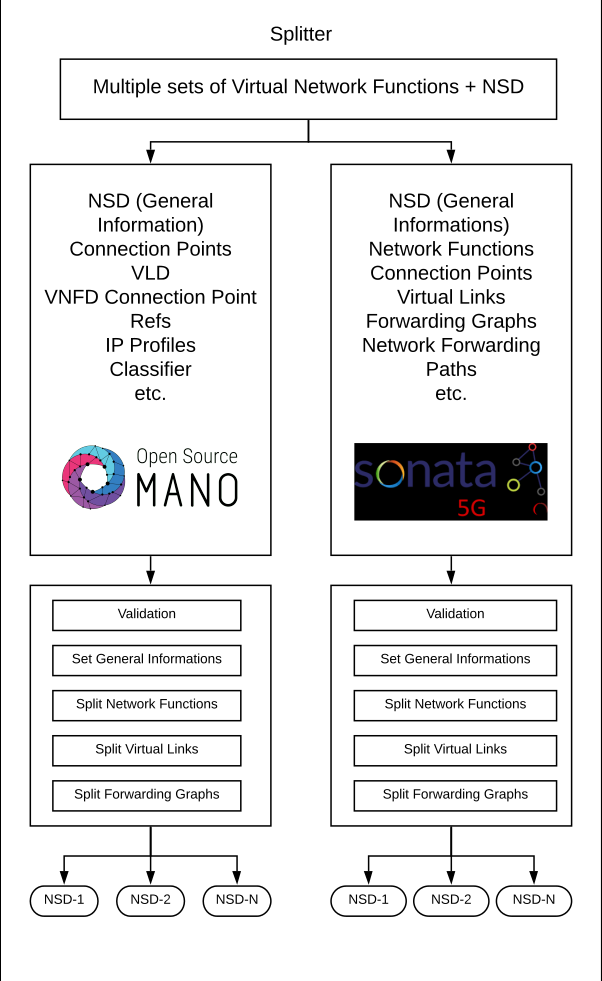
\includegraphics[width=0.5\linewidth]{figures/splitter}
	\caption{Scramble Architecture}
	\label{fig:splitter}
\end{figure}
